\documentclass[12pt,letterpaper]{article}
\usepackage{amsmath,amsthm,amsfonts,amssymb,amscd}
\usepackage{fullpage}
\usepackage{graphicx}
\usepackage{lastpage}
\usepackage{listings}
\lstset{
	numbers=left,
	numbersep=5pt,
	stepnumber=1,
	tabsize=2,
	showstringspaces=false
}
\usepackage{enumerate}
\usepackage{fancyhdr}
\usepackage{hyperref}
\usepackage{mathrsfs}
\usepackage{cancel}
\usepackage{xcolor}
\usepackage[margin=3cm]{geometry}
\setlength{\parindent}{0.0in}
\setlength{\parskip}{0.05in}

% Edit these as appropriate
\newcommand\course{STA561/CS571}
\newcommand\semester{Fall 2013}     % <-- current semester
\newcommand\hwnum{7}                  % <-- homework number
\newcommand\yourname{Matt Dickenson} % <-- your name
\newcommand\login{mcd31}           % <-- your NetID
\newcommand\hwdate{Due: 11 November, 2013}           % <-- HW due date

\newenvironment{answer}[1]{
  \subsubsection*{Problem #1}
}


\pagestyle{fancyplain}
\headheight 35pt
\lhead{\yourname\ \texttt{\login}\\\course\ --- \semester}
\chead{\textbf{\Large Homework \hwnum}}
\rhead{\hwdate}
\headsep 10pt

\begin{document}

\noindent \emph{Homework Notes:} I did not work with anyone else on this homework or refer to resources other than the course notes, textbook, and course Piazza page.

\begin{answer}{1}

\paragraph{A} 

\paragraph{B}

\end{answer}


\begin{answer}{2}

\paragraph{A} We expect values of $\pi_j$ (with $K=3$ for this example) close to $(1,0,0), (0,1,0)$, or $(0,0,1)$ with high probability, but assign very low probbaility to $pi_j=(\frac{1}{3}, \frac{1}{3}, \frac{1}{3})$.

\paragraph{B} In this case, $\pi_j$ is uniform.

\paragraph{C} When $\alpha = 10$, we assign high probability to $\pi_j=(\frac{1}{k}, \frac{1}{k}, ...)$.

\paragraph{D} Figure \ref{betasamps} presents 1,000 samples from three different parameterizations of the Beta distribution: $(0.2, 0.2), (1,1)$, and $(10,10)$. These samples support the answers above. For the first panel (Beta$(0.2, 0.2)$), samples of $0$ and $1$ are highly probable. In the second panel (Beta$(1,1)$), the samples appear to be uniformly distributed over the unit interval. Samples in the third panel (Beta$(10,10)$) favor values near the center of the distribution ($\frac{1}{k}=\frac{1}{2}$) rather than at the extremes of $0$ or $1$.

\begin{figure}[h!]
\begin{center}
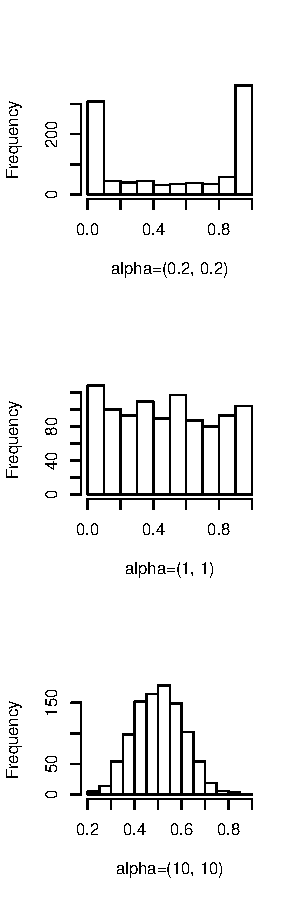
\includegraphics[scale=1]{betasamps.pdf}
\caption{1,000 Samples from Beta Distributions with Three Different Values of $\alpha$}
\label{betasamps}
\end{center}
\end{figure}

\paragraph{E} I suspect that inference in these models is easier with values of $\alpha$ similar to $[\alpha_1, ..., \alpha_k]=0.2$. Inference with this setting is easier because each document is assigned to a single topic with high probability, rather than a mixture of topics. That is, assigning $z_{i,j}$ is easier when $[\alpha_1, ..., \alpha_k]<1$.

\end{answer}


\begin{answer}{3}
One major challenge in moving forward with my project has been deciding how to make daily event data commensurable with dyadic data about military disputes that includes a start and end date. The current solution, which I will like employ for the duration of the project, is to aggregate the event data into dyad-months and put the dispute data into the same format. I am currently working on selecting features to use in training the HMM model. 
\end{answer}


\end{document}